\documentclass[a4paper,12pt]{article} 
% Paquetes......................................................................
\usepackage{amsmath, amssymb, amsfonts, latexsym}
\usepackage[utf8]{inputenc}
\usepackage[T1]{fontenc}
\usepackage{palatino}
\usepackage[full]{textcomp}
\usepackage{hyperref}
\usepackage{eurosym}
\usepackage[makeroom]{cancel}
\usepackage{array}
\usepackage{pdfpages}
\usepackage{float} % para que las figuras no floten
\usepackage{subcaption}
\usepackage{soul} % para el highlight \hl
\usepackage{pdfpages} % para pegar otro pdf dentro de este

\textheight = 24 cm
\textwidth = 17 cm

\renewcommand{\arraystretch}{1.25}
\renewcommand{\contentsname}{Contenidos}


% INICIO DEL DOCUMENTO --------------------------------------------------------
\begin{document}
	
	\setlength{\parindent}{0.5cm}
	\setlength{\voffset}{-2cm}
	\setlength{\hoffset}{-2cm}
	
	%%%%%%%%%%%%%%%%%%%%%%%%%%%%%%%%%%%%%%%%%
% Academic Title Page
% LaTeX Template
% Version 2.0 (17/7/17)
%
% This template was downloaded from:
% http://www.LaTeXTemplates.com
%
% Original author:
% WikiBooks (LaTeX - Title Creation) with modifications by:
% Vel (vel@latextemplates.com)
%
% License:
% CC BY-NC-SA 3.0 (http://creativecommons.org/licenses/by-nc-sa/3.0/)
% 
% Instructions for using this template:
% This title page is capable of being compiled as is. This is not useful for 
% including it in another document. To do this, you have two options: 
%
% 1) Copy/paste everything between \begin{document} and \end{document} 
% starting at \begin{titlepage} and paste this into another LaTeX file where you 
% want your title page.
% OR
% 2) Remove everything outside the \begin{titlepage} and \end{titlepage}, rename
% this file and move it to the same directory as the LaTeX file you wish to add it to. 
% Then add \input{./<new filename>.tex} to your LaTeX file where you want your
% title page.
%
%%%%%%%%%%%%%%%%%%%%%%%%%%%%%%%%%%%%%%%%%

%----------------------------------------------------------------------------------------
%	PACKAGES AND OTHER DOCUMENT CONFIGURATIONS
%----------------------------------------------------------------------------------------


%----------------------------------------------------------------------------------------
%	TITLE PAGE
%----------------------------------------------------------------------------------------

\begin{titlepage} % Suppresses displaying the page number on the title page and the subsequent page counts as page 1
	\newcommand{\HRule}{\rule{\linewidth}{0.5mm}} % Defines a new command for horizontal lines, change thickness here
	
	\center % Centre everything on the page
	
	%------------------------------------------------
	%	Headings
	%------------------------------------------------
	
	\textsc{\Large Máster en Inteligencia Artificial}\\[1.5cm] % Main heading such as the name of your university/college
	
	\textsc{\LARGE Ingeniería Ontológica}\\[0.5cm] % Major heading such as course name
	
	%\textsc{\large Minor Heading}\\[0.5cm] % Minor heading such as course title
	
	%------------------------------------------------
	%	Title
	%------------------------------------------------
	
	\HRule\\[0.4cm]
	
	{\huge\bfseries Diseño de una ontología para instalaciones deportivas}\\[0.4cm] % Title of your document
	
	\HRule\\[1.2cm]
	
	%------------------------------------------------
	%	Author(s)
	%------------------------------------------------
	
	%\begin{minipage}{0.4\textwidth}
	%	\begin{flushleft}
	%		\large
	%		\textit{Author}\\
	%		\textsc{Aída Muñoz Monjas} % Your name
	%	\end{flushleft}
	%\end{minipage}
	%~
	%\begin{minipage}{0.4\textwidth}
	%	\begin{flushright}
	%		\large
	%		\textit{Supervisor}\\
	%		Dr. Caroline \textsc{Becker} % Supervisor's name
	%	\end{flushright}
	%\end{minipage}
	
	% If you don't want a supervisor, uncomment the two lines below and comment the code above
	{\Large\textit{Authors}}\\
	
	{\large\textsc{Luis Couto seller\\
			 Irene Marbán Álvarez\\
			 Aída Muñoz Monjas} } % Your name
	
	%------------------------------------------------
	%	Date
	%------------------------------------------------
	
	\vfill\vfill\vfill % Position the date 3/4 down the remaining page
	
	{\large\today} % Date, change the \today to a set date if you want to be precise
	
	%------------------------------------------------
	%	Logo
	%------------------------------------------------
	
	%\vfill\vfill
	%\includegraphics[width=0.2\textwidth]{placeholder.jpg}\\[1cm] % Include a department/university logo - this will require the graphicx package
	 
	%----------------------------------------------------------------------------------------
	
	\vfill % Push the date up 1/4 of the remaining page
	
\end{titlepage}

%----------------------------------------------------------------------------------------

%\end{document}

	
	\tableofcontents
	
\newpage

	\section{Introducción}
	% Introduction. High level overview of the ontology you plan to develop and brief description of the datasets and web pages that you plan to use.
	
	El objetivo de este trabajo es diseñar e implementar una ontología que represente de manera correcta instalaciones deportivas y sus características y acciones relacionadas. Las ontologías y otras fuentes de conocimiento utilizadas durante el desarrollo de este trabajo serán citadas, y se puede acceder a ellas a través de los hipervínculos de la bibliografía.
	
	\section{Metodología NeOn}
	% Make a short overview of the NeOn methodology making explicit:
	%   a. which scenarios you plan to follow
	%   b. which activities from the glossary of activities you plan to execute in your ontology development project
	
	\section{Especificación de la ontología}
	% Ontology specification. You should include a complete ontology specification requirement document using the template explained during the lectures. The goal of the ontology should be clear enough. The document should include relevant competency questions and their answers.
	
	\section{Planificación temporal de la ontología}
	% Ontology Schedule. You should identify the ontology life cycle model you use in your ontology development. Activities should come from the glossary of terms. Include a Gantt chart with the planned activities.
		
	El ciclo de vida utilizado en el diseño y desarrollo de esta ontología es el ciclo de vida incremental, pudiéndose considerarse como el primer sprint (ciclo) de un modelo ágil.
	
	Se decidió utilizar un ciclo de vida incremental debido a las características del proyecto. 
	
	La planificación
	
	\section{Búsqueda de ontologías de alto nivel}
	% Search for existing top level and domain ontologies that you plan to reuse when building your ontology. Explain if you need to reuse the ontology as a whole or if you need some modules or statements. Explain in which repositories you made the search, ontologies found, their relevance to your work and the criteria being used for selecting or withdrawing some of them.
	
	\section{Recursos no ontológicos}
	%Search for non ontological resources and other terminologies that could be transformed into ontologies. Keep track of the URLs where you found them. For the selected resources, do not forget to justify why you have selected them. Check if you have Access rights for using them within your hands-on assigment.
	
	Una de las fuentes de información utilizadas para generar la ontología propuesta en este documento es el siguiente informe \cite{pdf-culturaydeporte}. A partir de este recurso no ontológico, mediante el uso de un T-Box se pudo realizar una modelización de la información descrita que representa la estructura taxonómica del documento en esta ontología de instalaciones deportivas. 
	
	El documento \cite{pdf-culturaydeporte} del Ministerio de Cultura y Deporte del Gobierno de España, contiene los  principales resultados del informe de explotación estadística del censo de instalaciones deportivas de 2005, así como las definiciones de las diferentes clases de instalaciones deportivas consideradas durante el censo.
	
	Al plasmar el conocimiento presente en este documento en el modelo de la ontología mediante un T-Box, se decidió mantener las clases intermedias presentes en el documento como parte de la ontología pese a que serán probablemente rara vez utilizadas para mantener la estructura del documento mencionado y facilitar la reutilización de este. 
	
	\begin{figure}[H]
		\centering
		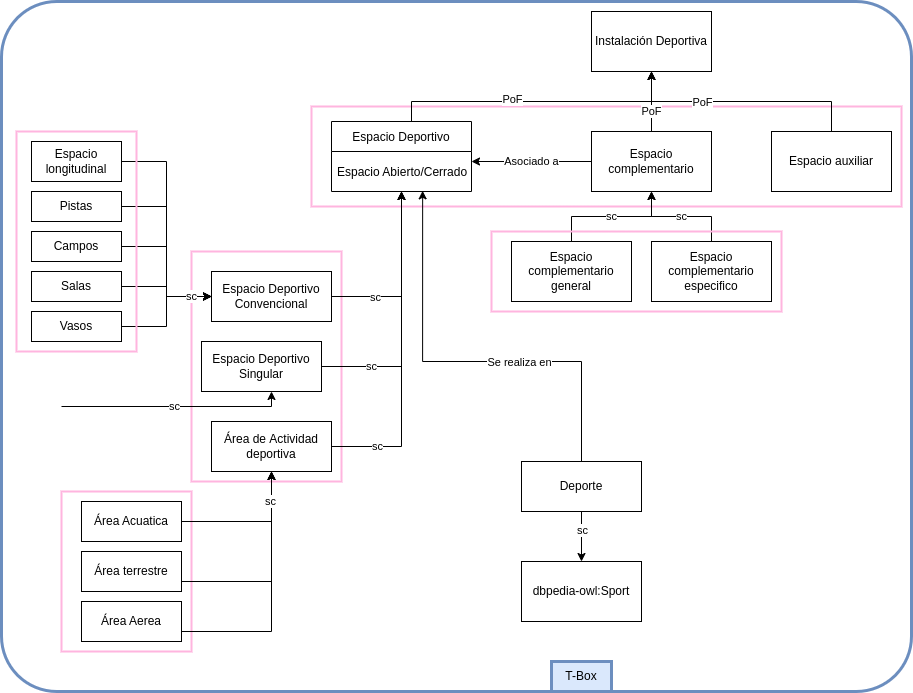
\includegraphics[width=0.7\textwidth]{include/tbox.png}
		\caption{Sección correspondiente a los recursos no ontológicos en la ontología.}
	\end{figure}
	
	Es importante señalar que la estructura taxonómica del documento descrito exige desambiguar entre las relaciones "sub-clase de" (\textit{sc} en el diagrama) y "parte de" (\textit{PoF} en el diagrama).
	
	\section{Patrones en la ontología}
	% Search for some ontology design patterns in the ontology design pattern portal that could be reused in your development.
	
	Para facilitar el diseño de los servicios ofrecidos por la organización en una instalación deportiva, se reutilizó el patrón de una relación N-aria según lo visto en clase. Este patrón se utiliza para representar una relación N-aria en el que todos los elementos tienen la misma importancia. Para representar esta relación N-aria se crea una clase, en nuestra ontología la clase \textit{ServicioOfrecido}, a la que asociar todos los atributos de la relación.
	
	\begin{figure}[H]
		\centering
		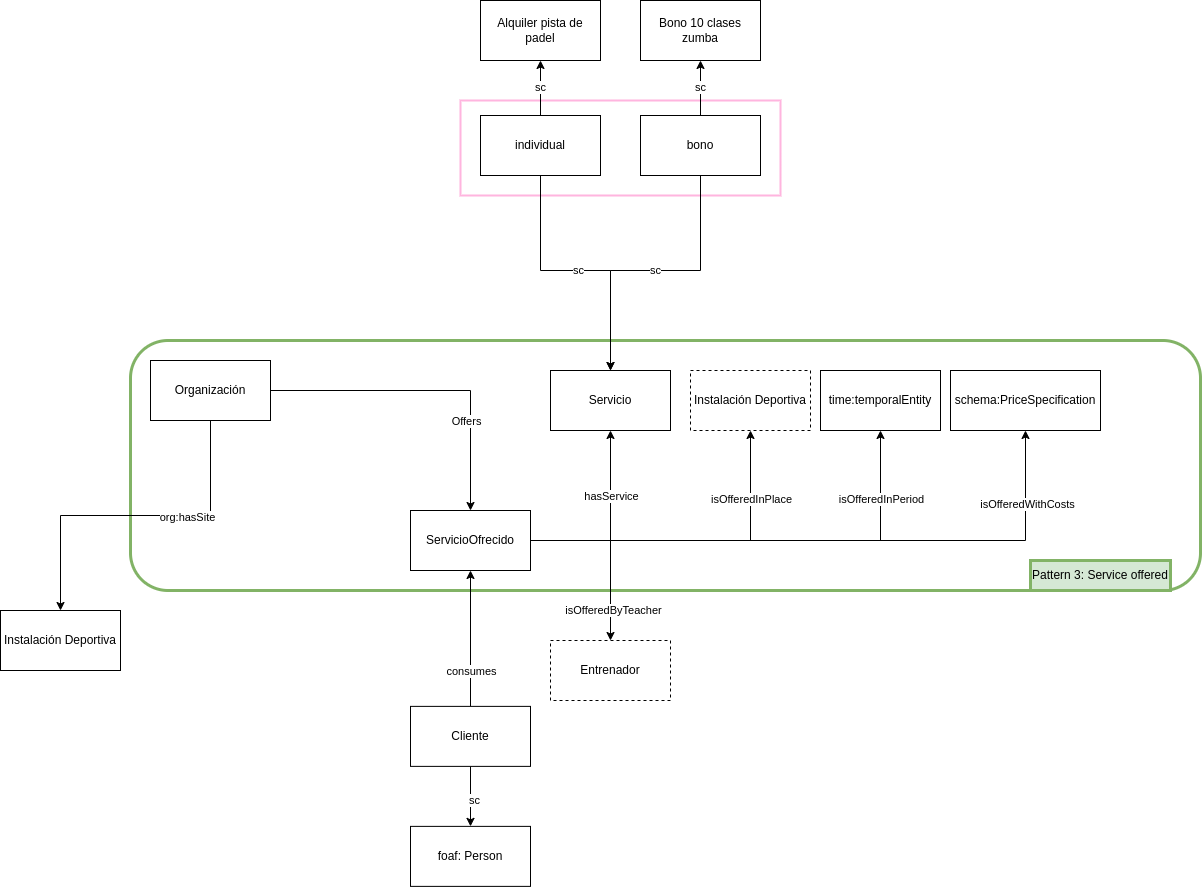
\includegraphics[width=0.5\textwidth]{include/patron.png}
		\caption{Sección correspondiente a los patrones utilizados en el diseño de la ontología.}
	\end{figure}
	
	
	\section{Modelo conceptual}
	% Build a conceptual model that integrates outcomes from the previous sections (c,d,e). This is the most important part of the work you are doing. Try to use:
	%  	i. Top level ontologies and other well-known ontologies. Classify in the pyramid of ontologies (figure use vs reuse) each of the ontologies that you reuse.
	%   ii. Transform each non-ontology resource into an ontology by using the T-box, A-Box or Population.
	%   iii. Select some Ontology Design Patterns (events, sequence, etc.)
	%   iv. Build the conceptual model of your ontology by integrating the above sources. The conceptual model should have at least 40 concepts, several subclass-of relations, disjoint, part-of (if needed), and ad-hoc relations.
	
	\section{Clases Multilingües}
	
	\section{Implementación de la ontología con OWL}
	% Implement the ontology in an ontology development tool, or other ontology editor, using OWL as ontology language
	
	\section{Evaluación de la ontología con OOPS!}
	% Evaluate the ontology with OOPS! and include in your report the pitfalls found. It is highly advisable to combine this evaluation with other ontology evaluation techniques.
	\cite{oops}
	
	\section{Evaluación. Mejoras propuestas}
	% Improve your ontology (conceptual model and implementation) taking into account the suggestions given by OOPS!. Iterate in these steps until the ontology pass most of the OOPS! recommedations.
	
	\section{Documentación de la ontología}
	% Document the ontology with Widoco and use Ontoology if required
		
	\cite{widoco}
	
	%\includepdf[pages=-]{include/documentation-widoco.pdf}
	
	\section{Conclusiones}
	
	
\newpage
	\section*{Bibliografía}
	\addcontentsline{toc}{section}{Bibliografía}
	\bibliography{include/references}
	\bibliographystyle{IEEEtran}

\end{document}